\documentclass[11pt,english,french]{scrreprt}
\usepackage{lmodern}
\usepackage{babel}
\renewcommand{\familydefault}{\rmdefault}
\usepackage[T1]{fontenc}
\usepackage{ucs}
\usepackage[utf8x]{inputenc}
\usepackage[a4paper]{geometry}
\geometry{verbose,tmargin=2cm,bmargin=2cm,lmargin=2cm,rmargin=2cm,headheight=2cm,footskip=1cm}
\setlength{\parskip}{\smallskipamount}
\setlength{\parindent}{0pt}

\usepackage{amsthm}
\usepackage{booktabs}
\usepackage{amsmath}
\usepackage[unicode=true, pdfusetitle,
 bookmarks=true,bookmarksnumbered=false,bookmarksopen=false,
 breaklinks=false,pdfborder={0 0 1},backref=false,colorlinks=false]
 {hyperref}

\makeatletter
\usepackage{colortbl}
\usepackage{color}
\usepackage[dvipsnames]{xcolor}
\usepackage{wrapfig}
\usepackage{graphicx}
\usepackage{listings}
\usepackage[calcwidth]{titlesec}
\usepackage{fix-cm}
\usepackage{multicol}
\usepackage{verbatim}
\usepackage{moreverb}
\usepackage{nicefrac}
\usepackage{amssymb}
\usepackage{array}
\usepackage{tabularx}
\usepackage{subfig}
\usepackage[french,ruled,vlined]{algorithm2e}
\SetAlgoProcName{Procédure}{proc}

\theoremstyle{remark}
  \newtheorem*{rem*}{Remarque}
  \newtheorem*{ex*}{Exemple}
\theoremstyle{definition}
  \newtheorem*{defi}{Définition}
  \newtheorem{ques}{Question}[section]
  \newtheorem{idee}{Idée}[ques]
  \newtheorem*{rap}{Rappel}

\definecolor{MyDarkBlue}{rgb}{0,0.08,0.45}

\lstset{language=C,
	 	basicstyle=\small\ttfamily,
		keywordstyle=\small\ttfamily,
		identifierstyle=,
		commentstyle=\textcolor{OliveGreen},
		columns=fullflexible,
		stringstyle=\small\ttfamily,
		showstringspaces=false,numberstyle=\tiny, breaklines=false, tabsize=4}

\titleformat{\section}[hang]{\sffamily\bfseries}
 {\Large\thesection}{12pt}{\Large}[{\titlerule[0.5pt]}]

\def\thickhrulefill{\leavevmode \leaders \hrule height 1pt\hfill \kern \z@}
\renewcommand{\maketitle}{\begingroup%
    \let\footnotesize\small
    \let\footnoterule\relax
    \parindent \z@
    \reset@font
    \begin{flushleft}
      \huge \sffamily \bfseries\color{orange} \@title
    \end{flushleft}
    \hrule height 1pt
    \begin{flushright}
      \large\sffamily\color{MyDarkBlue}\@author
    \end{flushright}
  \endgroup%
  \setcounter{footnote}{0}%
}

\AtBeginDocument{
  \def\labelitemi{\normalfont\bfseries{--}}
}

\makeatletter
\renewcommand\thesection{\arabic{section}}
\@addtoreset{section}{chapter}
\makeatother

\makeatother
\begin{document}
	
\title{LI310 - Examen 2010\\
Mardi 4 janvier 2011}
\author{Benjamin BARON}

\maketitle

\section{Cours} % (fold)

\begin{ques}
	Différence entre la cryptographie à clé secrète et la cryptographie à clé publique.
\begin{description}	
	\item [Cryptographie à clé secrète]
	Il y a une seule clé (la clé secrète) partagée entre les utilisateurs à la fois pour le chiffrement et le déchiffrement.
	\begin{ex*}
		La cryptographie à clé secrète est utilisée dans 802.11 avec WEP.
	\end{ex*}
	\item [Cryptographie à clé publique]
	Il y a une seule paire de clés :\begin{itemize}
		\item Clé publique : clé non secrète utilisée pour le chiffrement ;
		\item Clé privée : clé secrète utilisée pour le déchiffrement.
	\end{itemize}
	\begin{ex*}
		La cryptographie à clé publique est utilisée dans GSM.
	\end{ex*}
\end{description}
\end{ques}

\begin{ques}
	L'avantage de la cryptographie à clé publique réside dans la facilité de distribution de la clé publique de chiffrement.
	
	Dans la cryptographie à clé secrète, il y a une même clé partagée à la fois par le point d'accès et les terminaux, ce qui pose un problème pour sa diffusion.
\end{ques}

\begin{ques}
	Dans les réseaux 802.11, la sécurité WEP (\emph{Wired Equivalent Privacy}) se base sur la cryptographie à clé secrète. Une même clé WEP est partagée entre les terminaux et le point d'accès (généralement inscrite sur la box).
\end{ques}

\begin{ques}
	Schéma d'authentification avec WEP dans 802.11.
	
	\begin{figure}[h!]
		\center
		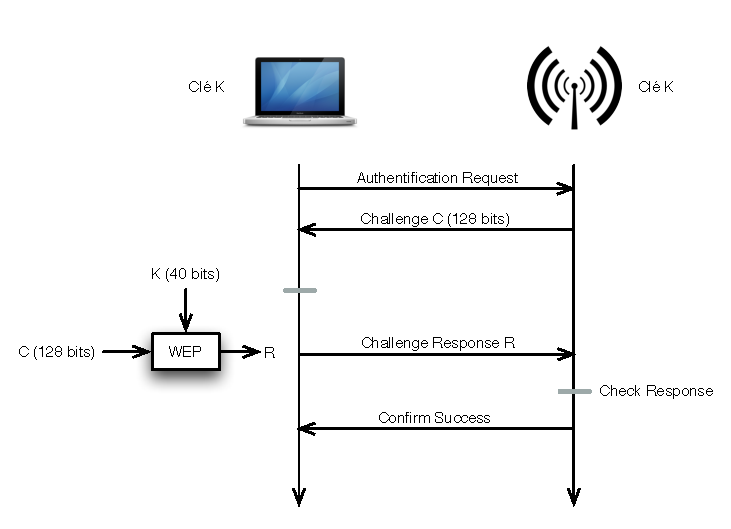
\includegraphics[scale=1]{Exam2009/WEP}
	\end{figure}
\end{ques}

\begin{ques}
	Dans la sécurité WEP, l'ICV (Integrity Check Value) calculé par l'algorithme CRC-32 est utilisé pour vérifier l'intégrité du message transmis entre deux terminaux. L'algorithme CRC-32 détecte des inversions de bits, qui vont être alors considérées comme frauduleuses.
\end{ques}

\clearpage

\section{Transmission de données} % (fold)

Un signal porteur d’information de fréquences strictement inférieures à $f_{max} = 10$ kHz est numérisé. Chaque échantillon est quantifié en utilisant une échelle qui possède 128 niveaux quantifiés, codés en binaire. Le message numérique binaire produit est transmis à l’aide d’un code NRZ $M$-aire.

\begin{ques}
	Si l'on veut minimiser le débit binaire du message numérique produit à l'issue de l'opération de numérisation, d'après le théorème d'échantillonnage de Shannon, on a :\[f_e >2f_{max}\Rightarrow f_e=20\;\textrm{kHz}\]
\end{ques}

\begin{ques}
	Pour permettre la transmission de ce message numérique, la capacité $C$ du canal de transmission doit vérifier :\[C\geqslant D_{source} = \frac{\textrm{Nb bits / échantillon}}{T_e} = \textrm{Nb bits / échantillon} \times f_e = \log_2(128)\times 20.10^3 = 140\;\textrm{kbit/s}\]
\end{ques}

\begin{ques}
	Le canal de transmission possède une largeur de bande passante $B$ égale à 90 kHz. Afin d’autoriser l’usage d’un code détecteur d’erreur, la transmission doit s’effectuer à un débit binaire $D_b$ de 200 kbit/s.
	
	Calcul du rapport signal à bruit $\left(\nicefrac{S}{N}\right)_{dB}$ minimal nécessaire en réception.
	
	La capacité $C$ du canal de transmission est telle que $C\geqslant D_b$.
	
	Or d'après la loi de Shannon, la capacité $C$ est égale à :
	\begin{eqnarray*}
	C=B\log_{2}\left(1+\frac{P_{S}}{P_{N}}\right) & \geqslant & D_{b}\\
	\frac{P_{S}}{P_{N}} & \geqslant & 2^{\nicefrac{D_{b}}{B}}-1\\
	\left(\nicefrac{S}{N}\right)_{dB} & \geqslant & 10\log_{10}\left(2^{\nicefrac{D_{b}}{B}}-1\right)\textrm{ car }\left(\nicefrac{S}{N}\right)_{dB}=10\log_{10}\left(\frac{P_{S}}{P_{N}}\right)\\
	\left(\nicefrac{S}{N}\right)_{dB} & \geqslant & 10\log_{10}\left(2^{\nicefrac{200}{90}}-1\right)=5,64\;\textrm{dB}\end{eqnarray*}
\end{ques}

\begin{ques}
	Supposons le rapport signal à bruit suffisant. 
	
	D'après la loi de Nyquist, on a \[R_S \leqslant 2b\log_2(M)\Leftrightarrow M\geqslant 2^{\nicefrac{D_b}{2B}}=2,16\]
	
	Or la valence $M$ est une puissance de 2, donc $M=2^2=4$.
	
	La durée $T_S$ des symboles est exprimée par :\[T_S=\frac{\log_2(M)}{D_b}=\frac{\log_2(4)}{200.10^3}=10\;\mu\textrm{s}\]
\end{ques}

\begin{ques}
	On souhaite augmenter la portée de la liaison. Le rapport signal à bruit en réception est alors de 2,4 dB. On se propose alors de diminuer le nombre $n$ de niveaux de quantification du numérisateur de manière à ce que la transmission reste faisable.
	
	On a la relation :\[D_{source} =f_e\times \log_2(n)\leqslant C=B\log_2\left(1+\frac{P_S}{P_N}\right)\]
	Or \[\left(\nicefrac{S}{N}\right)_{dB}=10\log_{10}\left(\frac{P_S}{P_N}\right)\Leftrightarrow\frac{P_S}{P_N}=10^{\frac{\left(\nicefrac{S}{N}\right)_{dB}}{10}}\]
	\[\Leftrightarrow \log_2(n)\leqslant \frac{B}{f_e}\log_2\left(1+10^{\frac{\left(\nicefrac{S}{N}\right)_{dB}}{10}}\right)\]
	\[\Leftrightarrow n\leqslant 2^{\nicefrac{B}{f_e}\log_2\left(1+10^{\frac{\left(\nicefrac{S}{N}\right)_{dB}}{10}}\right)} = 92,66\]
	
	Ainsi, $n=64=2^6$ niveaux de quantification.
\end{ques}

\clearpage

\section{HDLC} % (fold)

Un équipement de transmission A situé sur un satellite dialogue avec un autre équipement B au sol à l’aide d’une liaison utilisant le protocole LAP-B (variante de HDLC). Le satellite se situe à $d = 36\,000$ km d’altitude. On considère que les temps de traitement des données (constitution et réception des trames) sont négligeables et que toute trame de données est instantanément acquittée.

On suppose que seul le transmetteur A situé sur le satellite envoie des données et que les trames émises en continu les unes à la suite des autres contiennent toutes un fanion de début et de fin. Toutes les trames sont acquittées individuellement.	8 La vitesse de propagation du signal est d’environ $c = 3.10^8$ m/s. La taille du champ de données de la trame est ici de 128 octets, l’entête du protocole est codé sur 56 bits et la liaison a un débit $D_b$ de 64 kbit/s.

\begin{ques}
	Temps $T$ durant lequel l'émetteur A devra conserver une trame dans son buffer en émission si l’on considère que les transmissions se font sans erreur et qu’une trame est transmise dès qu’elle est prête à être envoyée.
	
	\[T = t_t + 2t_p + t_{ACK}\]
	
	Temps de transmission $t_t$ d'une trame de données :\[t_t = \frac{L_{trame}}{D_b} = \frac{L_{data}+L_{header}}{D_b} = \frac{128\times 8+56}{64.10^3} = 16,875\;\textrm{ms}\]
	
	Temps de transmission $t_{ACK}$ d'une trame ACK :\[t_{ACK} = \frac{L_{ACK}}{D_b} = \frac{56}{64.10^3} = 0,875\;\textrm{ms}\]
	
	Temps de propagation $t_p$ entre A et B : \[t_p = \frac{d}{c} = \frac{36\,000.10^3}{3.10^8} = 120\;\textrm{ms}\]
	
	Ainsi, $T = t_t + 2t_p + t_{ACK} = 16,875 + 0,875 + 240 = 257,75$ ms.
\end{ques}

\begin{ques}
	Taille minimale $W_{min}$ de la fenêtre d'anticipation du satellite pour que la transmission soit la plus efficace possible.
	
	Il faut que, avant la fin de la transmission des $W_{min}$ trames consécutives, on ait reçu l'ACK de la première trame :\[W_{min}.t_t \geqslant T\Leftrightarrow W\geqslant \frac{T}{t_t} \geqslant 15,25\]
	
	Ainsi, $W_{min} = 16$. 
\end{ques}

\begin{ques}
	Relation entre la taille $W$ de la fenêtre d'anticipation et le nombre $n$ de bits sur lequel est codé le numéro de séquence de la trame.
	
	Il faut que le nombre de valeur (numéro de séquence) que l'on peut adresser avec $n$ éléments binaires (bits) soit supérieur à $W$. Ainsi, $2^n\geqslant W$.
\end{ques}

\begin{ques}
	Dans HDLC, il est spécifié que le numéro de trame est codé sur 3 ou 7 bits. D'après les questions 2 et 3, on a $16 \leqslant W\leqslant 2^n$.\begin{itemize}
		\item Si $n=3$, alors $16\leqslant W\leqslant 8$ : impossible
		\item Si $n=7$, alors $16\leqslant W\leqslant 128$ : possible
	\end{itemize}
	La valeur $n=7$ conviendrait.
\end{ques}

\begin{ques}
	Compléter le schéma.
	
	\begin{figure}[h!]
		\center
		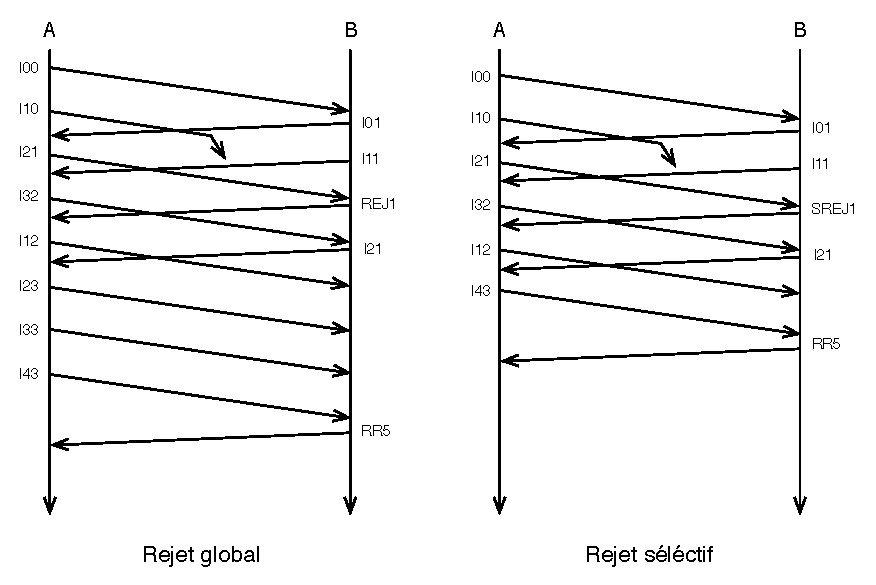
\includegraphics[scale=.8]{Exam2009/echange-hdlc}
	\end{figure}
\end{ques}

\clearpage

\section{Réseaux locaux et CSMA/CD} % (fold)
\begin{rap}
	Une station qui souhaite transmettre des données respecte les étapes suivantes :\begin{enumerate}
		\item Ecoute du canal pendant une durée équivalente à la transmission de 96 bits afin de s’assurer que le canal est libre.
		\item Si le canal est libre alors la machine transmet ses données.
		\item Si la machine détecte une collision, elle continue à émettre 32 bits (séquence de brouillage $t_{jam} = \nicefrac{32}{D_b} = 3,2\;\mu\textrm{s}$) puis cesse son émission, elle attend ensuite pendant un certain temps aléatoire (retrait exponentiel) et recommence à l’étape 1. L’algorithme de retrait exponentiel consiste à attendre un temps aléatoire compris entre 0 et $\min(2^i,,1023)$ intervalles de temps élémentaires (\emph{slot-time}) après la $i$-ème collision. Après 16 tentatives d’envoi échouées, l’émetteur abandonne.
	\end{enumerate}
\end{rap}
	  
	Dans les questions ci-dessous on suppose que lorsqu’une station veut transmettre, le canal est toujours libre (ce qui n’empêche pas les collisions par la suite). On prendra soin d’écrire le résultat sous forme littérale avant de passer à l’application numérique :\begin{itemize}
	\item Débit $D_b = 10$ Mbit/s
	\item Taille maximale du champ de données d’une trame Ethernet $L_{data} = 1500$ octets
	\item Longueur du câble $d = 2,5$ km
	\item Vitesse de propagation $c = 100\,000$ km/s
	\item Intervalle de temps élémentaire $TS = 51,2\;\mu\textrm{s}$
\end{itemize}

\begin{ques}
	Durée $T_{ecoute}$ correspondant au temps d'écoute obligatoire de l'étape 1 :\[T_{ecoute} = 96\times T_b = \frac{96}{D_b} = \frac{96}{10.10^6} = 96\;\mu\textrm{s}\]
\end{ques}

\begin{ques}
	Temps $t_t$ de transmission d'une trame Ethernet de taille maximale.
	\[t_t = (L_{data} + L_{header})\times T_b = \frac{L_{data} + L_{header}}{D_b} = \frac{(1500+26)\times 8}{10.10^6} = 1220,8\;\mu\textrm{s}\]
\end{ques}

\begin{ques}
	Temps $t_1$ qui s'écoule au minimum entre le moment où une machine veut envoyer une trame de taille maximale et le moment où la trame est intégralement reçue par le destinataire.
	\[t_1 = t_{ecoute} + t_t + t_p = 9,6 + 1220,8 + 25 = 1255,4\;\mu\textrm{s}\]
	En effet, le temps de propagation $t_p$ est égal à \[t_p = \frac{d}{c} = \frac{2,5}{100\,000} = 25\;\mu\textrm{s}\]
	\begin{rem*}
		On peut considérer $t_p = 0$ si la machine destinataire est proche de la machine émettrice.
	\end{rem*}
\end{ques}

\begin{ques}
	On suppose qu'il y a collision. Temps $t_2$ qui s'écoule au maximum entre le moment où une machine veut envoyer une trame et le moment où cette machine détecte la collision.
	\[t_2 = t_{ecoute} + 2\times t_p = 2\times 25 + 9,6 = 59,6\;\mu\textrm{s}\]
\end{ques}

\begin{ques}
	Temps $t_3$ qui s'écoule au maximum entre le moment où une machine veut envoyer une trame et le moment où la trame est intégralement reçue par le destinataire en supposant qu'il y a une seule collision.
	\begin{eqnarray*}
	t_{3} & = & t_{ecoute}+2t_{p}+t_{jam}+1\times TS+t_{ecoute}+t_{t}+t_{p}\\
	t_{3} & = & 59,6+3,2+51,2+1255,4=1369,4\;\mu\textrm{s}\end{eqnarray*}
\end{ques}

\begin{ques}
	On suppose qu'il y a une collision à chaque envoi. Temps $t_4$ qui s'écoule au maximum entre le moment où la machine veut envoyer une trame et le moment où la machine abandonne (16 échecs).
	\begin{eqnarray*}
	t_{4} & = & \sum_{i=1}^{15}\left(t_{ecoute}+2t_{p}+t_{jam}+\min\left(2^{i}-1,\,1023\right)\times TS\right)+t_{ecoute}+2t_{p}+t_{jam}\\
	 & = & 16\times\left(t_{ecoute}+2t_{p}+t_{jam}\right)+\left(1+3+7+15+31+63+127+255+511+1023\times6\right)\times TS\\
	t_{4} & = & 16\times\left(59,6+3,2\right)+7151\times51,2=367\,136\;\mu\textrm{s}\end{eqnarray*}
\end{ques}

\clearpage

\section{TCP} % (fold)

Echange considéré :
\begin{figure}[h!]
	\center
	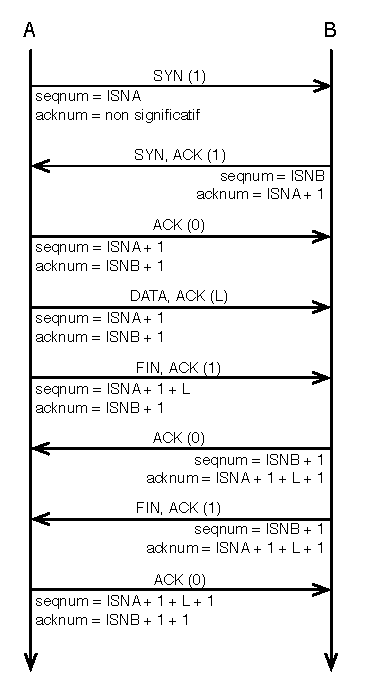
\includegraphics[scale=1]{Exam2009/echange-TCP}
\end{figure}

\begin{ques}
	ISN --- \emph{Initial Sequence Number} :\begin{itemize}
		\item Numéro de séquence initial (ISN) de A : \lstinline!DC:A5:2F:67! ;
		\item Numéro de séquence initial (ISN) de B : \lstinline!2D:00:2A:58!.
	\end{itemize}
\end{ques}

\begin{ques}
	Dans la trace, le segment de données (4\ieme trame) a été tronqué. Nombre $L$ d'octet que ce segment TCP transporte :\begin{itemize}
		\item Longueur du datagramme IP : champ \lstinline!Longueur totale! : 0x058C = 142 octets ;
		\item Longueur du header IP : champ \lstinline!IHL! : $5\times 4$ octets ;
		\item Longueur du header TCP : champ \lstinline!THL! : $8\times 4$ octets.
	\end{itemize}
	
	Ainsi, $L = 1420 - 20 - 32 = 1368$ octets.
\end{ques}

\begin{ques}
	Trace considérée.
	
	\begin{figure}[h!]
		\center
		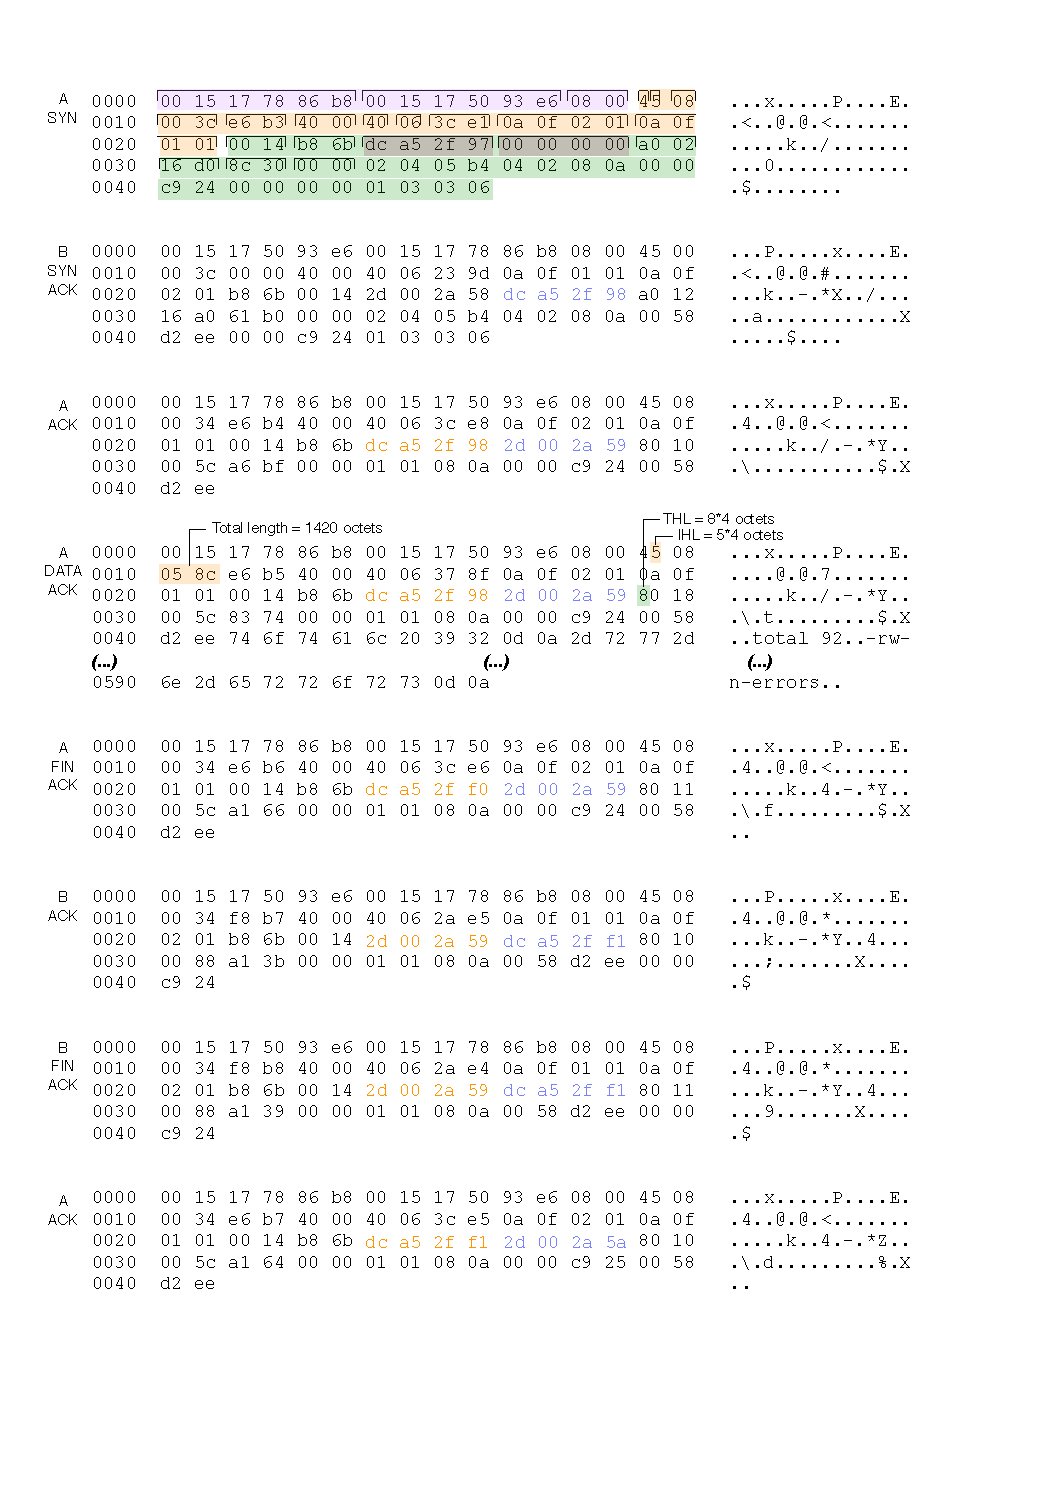
\includegraphics[scale=1.1]{Exam2009/trace}
	\end{figure}
\end{ques}

\end{document}